\documentclass[12pt,letterpaper]{article}

\usepackage[T1]{fontenc}
\usepackage[utf8]{inputenc}
\usepackage[spanish,mexico,es-tabla,es-noshorthands]{babel}
\usepackage{newtxtext,newtxmath}          % Times New Roman
\usepackage[margin=2.5cm]{geometry}
\usepackage{graphicx}
\usepackage{float}
\usepackage{caption}
\usepackage{subcaption}
\usepackage{booktabs}
\usepackage{enumitem}
\usepackage{amsmath}          % no cargar amssymb: choca con \Bbbk de newtxmath
\usepackage{listings}
\usepackage{xcolor}
\usepackage{setspace}
\usepackage[colorlinks=true,allcolors=black]{hyperref}
\usepackage{todonotes}                    % usar [disable] para la versión final

\graphicspath{{evidencias/}{../assets/}}
\captionsetup{labelsep=colon,font=small,labelfont=bf}
\onehalfspacing
\setlength{\parskip}{6pt}

% Títulos de sección al estilo del formato de la profesora
\usepackage{titlesec}
\titleformat{\section}{\normalfont\large\bfseries}{}{0pt}{}
\titleformat{\subsection}{\normalfont\normalsize\bfseries}{}{0pt}{}

\definecolor{codekw}{RGB}{0,0,180}
\definecolor{codecm}{RGB}{0,128,0}
\definecolor{codestr}{RGB}{170,0,0}
\definecolor{codebg}{RGB}{248,248,248}

\lstdefinestyle{hdl}{
  language=VHDL,
  basicstyle=\ttfamily\footnotesize,
  keywordstyle=\color{codekw}\bfseries,
  commentstyle=\color{codecm}\itshape,
  stringstyle=\color{codestr},
  backgroundcolor=\color{codebg},
  numbers=left, numberstyle=\tiny\color{gray}, numbersep=8pt,
  frame=single, rulecolor=\color{gray!50},
  breaklines=true, breakatwhitespace=true,
  tabsize=2, showstringspaces=false, captionpos=b,
  extendedchars=true, inputencoding=utf8,
  literate={á}{{\'a}}1 {é}{{\'e}}1 {í}{{\'i}}1 {ó}{{\'o}}1 {ú}{{\'u}}1
           {Á}{{\'A}}1 {É}{{\'E}}1 {Í}{{\'I}}1 {Ó}{{\'O}}1 {Ú}{{\'U}}1
           {ñ}{{\~n}}1 {Ñ}{{\~N}}1 {ü}{{\"u}}1 {¿}{{?`}}1 {¡}{{!`}}1
}
\lstset{style=hdl}
% Para que el código comparta numeración con las figuras (en vez de tener su propio
% contador "Listing"), NO usar caption=/label= dentro de lstlisting/lstinputlisting.
% En su lugar, envolver el listado en un \begin{figure} normal y poner \caption y
% \label ahí (\figurename ya es "Figura" por babel-spanish):
%   \begin{figure}[H]
%     \centering
%     \lstinputlisting[style=hdl]{codigo/archivo.vhd}
%     \caption{Descripción del código.}
%     \label{fig:archivo}
%   \end{figure}

\graphicspath{{evidencias/}{practica5/evidencias/}{../assets/}{assets/}}

\begin{document}

\begin{titlepage}
\centering
\noindent
\begin{minipage}[c]{0.45\textwidth}\centering
  
\includegraphics[height=3.2cm]{logo-unam.jpg}
\end{minipage}\hfill
\begin{minipage}[c]{0.45\textwidth}\centering
  
\includegraphics[height=3.2cm]{logo-fi.png}
\end{minipage}

\vspace{1.2cm}
{\Large\bfseries UNIVERSIDAD NACIONAL AUTÓNOMA\\[2pt] DE MÉXICO\par}
\vspace{0.9cm}
{\large\bfseries FACULTAD DE INGENIERÍA\par}
\vspace{0.6cm}
{\large\bfseries INGENIERÍA EN COMPUTACIÓN\par}
\vspace{0.6cm}
{\bfseries Laboratorio de Organización de Arquitectura de Computadoras\par}
\vspace{0.9cm}
{\bfseries Reporte - Construcción de máquinas de Estados usando memorias: Direccionamiento Implícito\par}

\vspace{1.0cm}
\raggedright
{\bfseries NOMBRE DE LOS INTEGRANTES:}\\
Omar Alfonso Zendejas Labias \quad Grupo de Teoría: 04\\
Emiliano García Olvera \quad Grupo de Teoría: 02

\vspace{1.0cm}
{\bfseries NOMBRE DEL PROFESOR: ING. KAREN PÉREZ}

\vspace{0.6cm}
{\bfseries GRUPO: 06 \quad EQUIPO: 9}

\vspace{0.6cm}
{\bfseries SEMESTRE:} \underline{2027-1.}

\vspace{0.6cm}
\hfill {\bfseries FECHA DE ENTREGA: 5 de octubre de 2026}
\thispagestyle{empty}
\end{titlepage}

\setcounter{page}{1}

\section{Objetivo}

Construir una máquina de estados finita a partir de una carta ASM utilizando una memoria
como elemento central del diseño, empleando el método de direccionamiento implícito. A
diferencia del direccionamiento por trayectoria y del direccionamiento entrada-estado, aquí la
dirección de memoria se forma únicamente con el estado presente. El estado siguiente se
determina con un contador que avanza en uno o carga el campo de liga, según el valor de la
variable sensada.

Para ello se diseñó una carta ASM de siete estados, tres entradas (X, Y y Z) y cuatro salidas
(dos con lógica estándar y dos con lógica negada), con salidas condicionales en cinco
decisiones. Se determinó el tamaño de la memoria, se obtuvo su contenido completo, se
implementó el sistema en VHDL sobre la tarjeta DE10-Lite mediante Quartus Prime, y se verificó
su funcionamiento por simulación y en hardware.

\section{Introducción}

En el direccionamiento implícito, la memoria no almacena dos ligas como en el método
entrada-estado, sino una sola \textbf{liga} de salto. Un campo de \textbf{prueba} selecciona
la variable de entrada que se sensa en el estado, y el campo \textbf{VF} (verdadero-falso)
indica el valor que debe tener esa variable para realizar el salto \cite{savage}.

Una compuerta XNOR compara la variable sensada (\textit{Q}) con VF. Si ambos valores coinciden,
se genera la señal de \textbf{carga}, y el contador toma el valor del campo de liga. Si no
coinciden, se genera la señal de \textbf{incremento} (una compuerta XOR entre Q y VF), y el
contador avanza al estado siguiente en secuencia. La relación se resume en la siguiente tabla.

\begin{center}
\begin{tabular}{@{}c c c c@{}}
\toprule
\textbf{VF} & \textbf{Q} & \textbf{Incrementa} & \textbf{Carga} \\
\midrule
0 & 0 & 0 & 1 \\
0 & 1 & 1 & 0 \\
1 & 0 & 1 & 0 \\
1 & 1 & 0 & 1 \\
\bottomrule
\end{tabular}
\end{center}

Como consecuencia, si una decisión no cumple la condición de salto, el estado siguiente debe ser
el código del estado presente más uno. Esto obliga a que las ramas de incremento apunten a
códigos consecutivos.

Las salidas condicionales se manejan desdoblando el campo de salidas en dos conjuntos: las
\textbf{salidas F}, activas cuando la variable sensada vale 0 (incremento), y las
\textbf{salidas V}, activas cuando vale 1 (carga). Un multiplexor de 2 a 1 selecciona entre
ambos conjuntos con la señal de carga.

El tamaño de la memoria se calcula con

\begin{equation}
\text{Memoria} = 2^{n} \times m
\label{eq:tam}
\end{equation}

donde $n$ es el número de bits de estado y $m$ el número de bits por localidad.

\section{Desarrollo}

\subsection{Planteamiento: carta ASM}

La carta ASM se diseñó primero a mano, como se muestra en la figura \ref{fig:evid-asm}. Después
se trasladó a la forma digital de la figura \ref{fig:asm}. Tiene siete estados (EST0 a EST6),
tres entradas (X, Y y Z) y cuatro salidas: $S_1$ y $S_2$ con lógica estándar, y $\overline{U_1}$
y $\overline{U_2}$ con lógica negada. En la carta, $\overline{U_1}$ y $\overline{U_2}$ aparecen
como U1 y U2 en el diseño manual.

\begin{figure}[H]
  \centering
  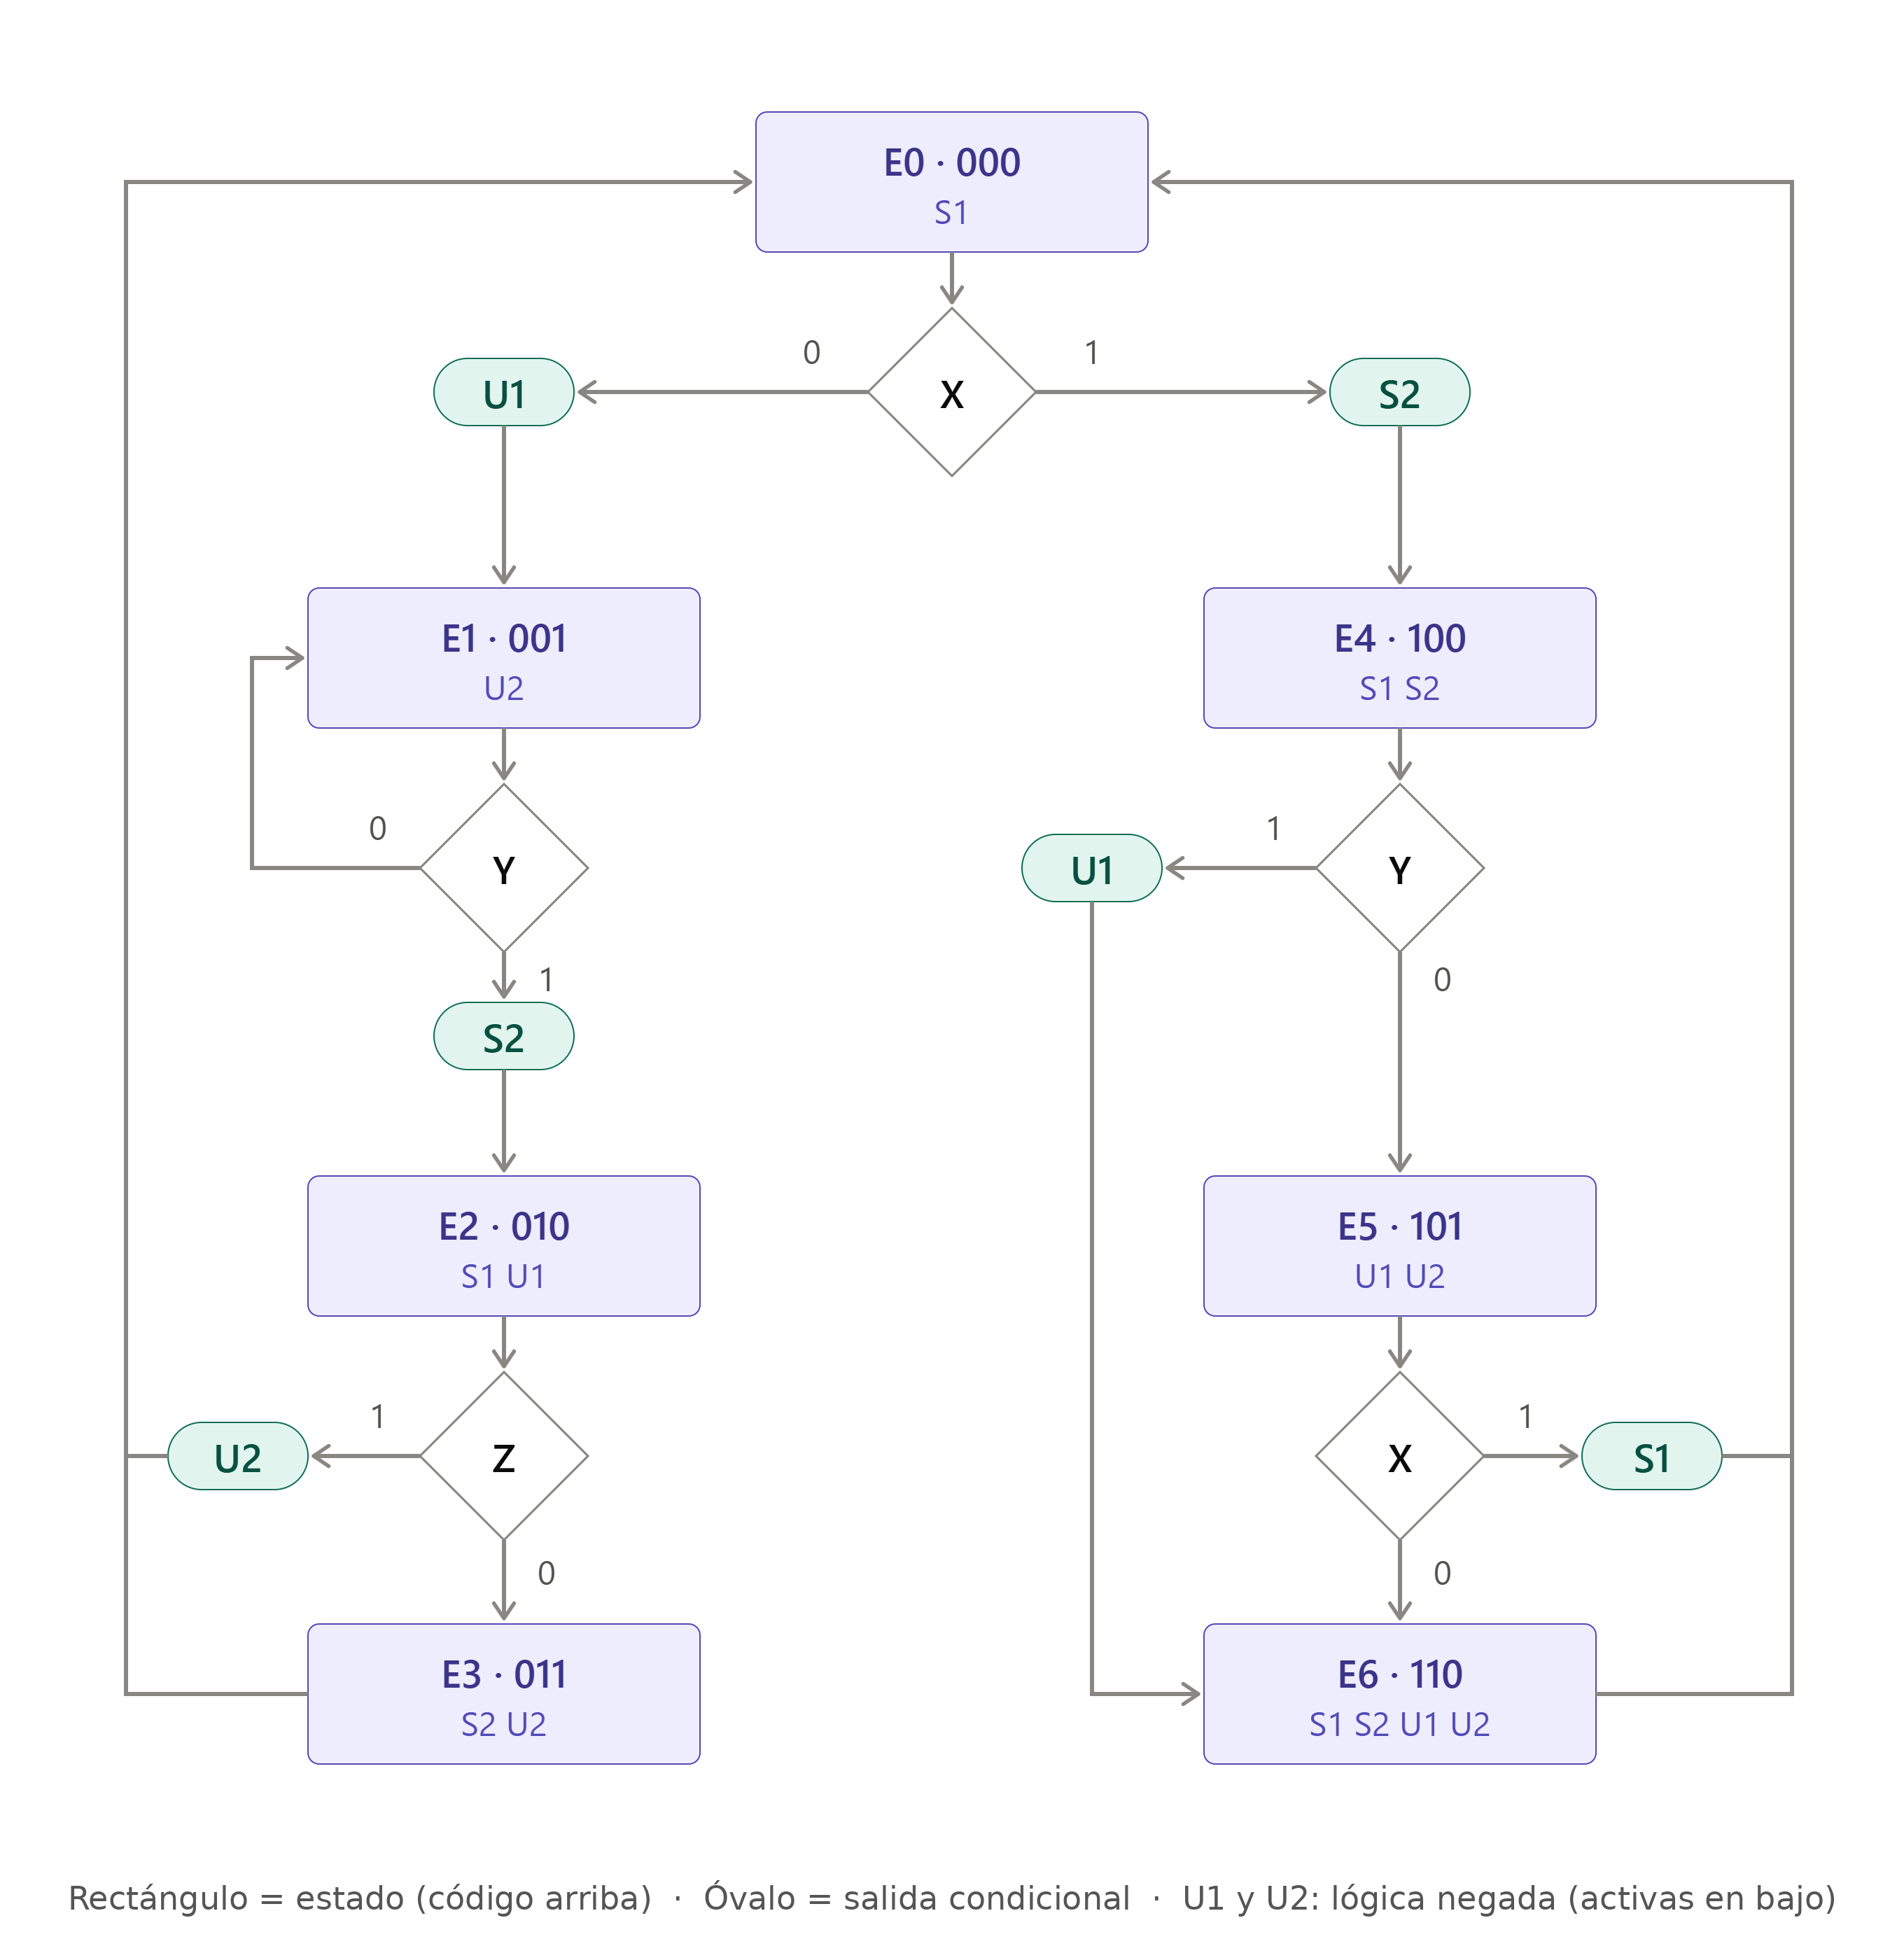
\includegraphics[width=0.78\textwidth]{01-carta-asm.png}
  \caption{Carta ASM propuesta: siete estados, tres entradas y cuatro salidas, con salidas
  condicionales en las decisiones de EST0, EST1, EST2, EST4 y EST5.}
  \label{fig:asm}
\end{figure}

\begin{figure}[H]
  \centering
  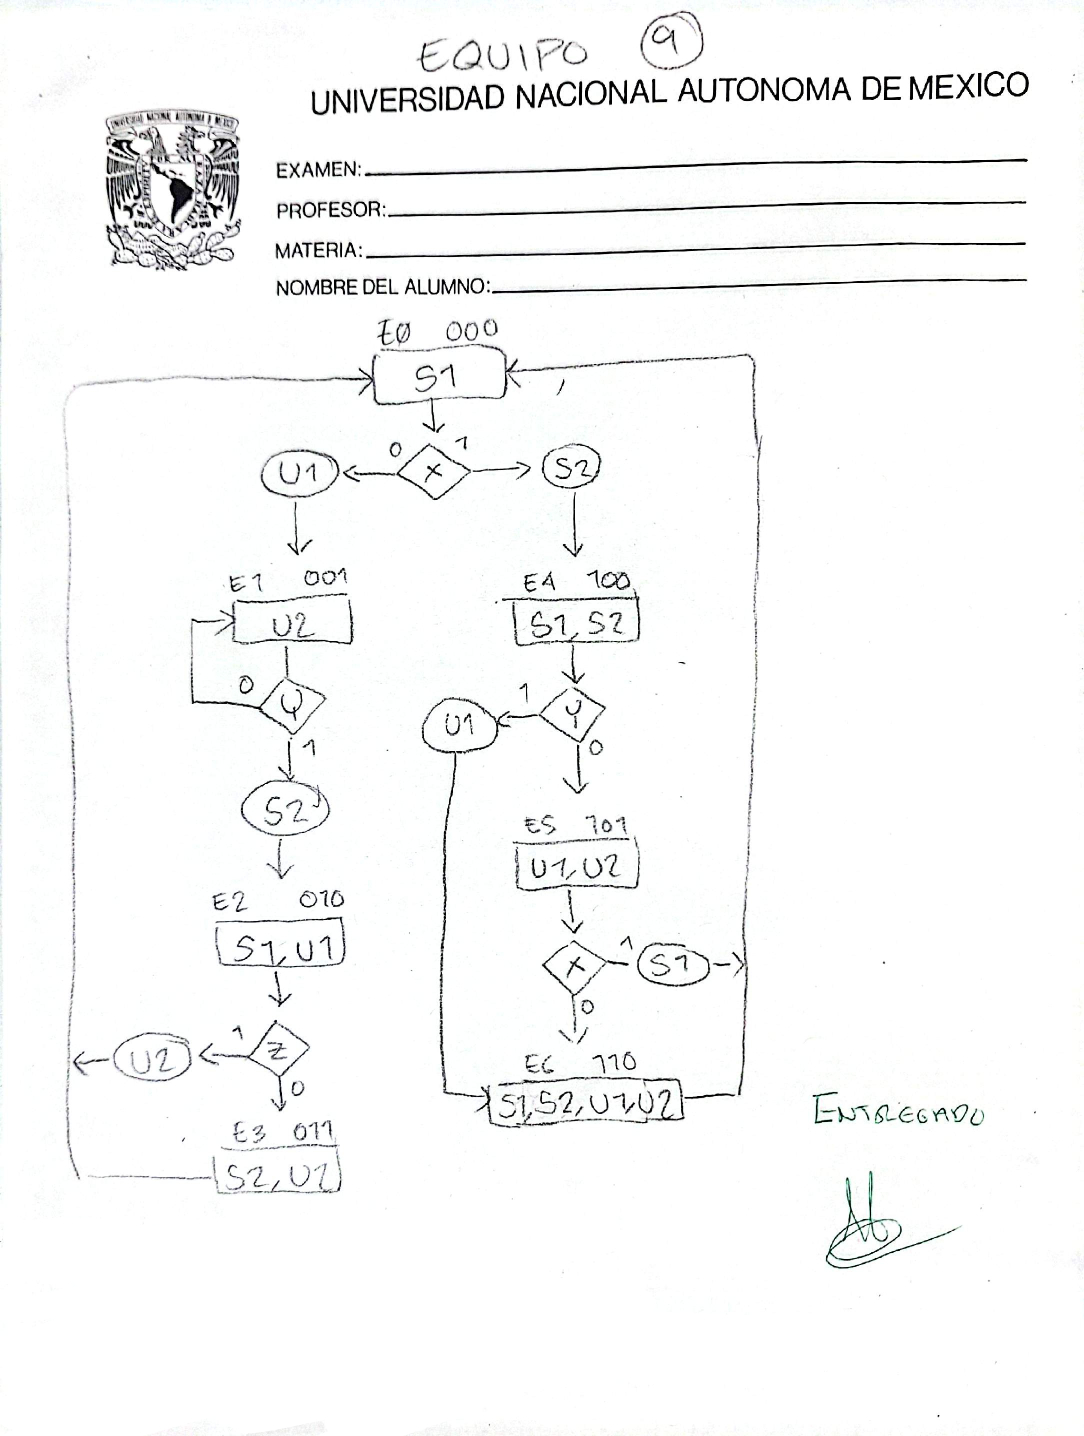
\includegraphics[width=0.9\textwidth,height=0.85\textheight,keepaspectratio]{evidencia-carta-asm.jpg}
  \caption{Evidencia del diseño manual de la carta ASM, con la asignación de códigos de estado.}
  \label{fig:evid-asm}
\end{figure}

Con siete estados se requieren $\lceil \log_2 7 \rceil = 3$ bits de estado, por lo que hay ocho
localidades y una dirección sin utilizar (\texttt{111}). La variable sensada se codifica en el
campo de prueba. Las transiciones incondicionales de EST3 y EST6 hacia EST0 se resuelven con una
prueba sobre la entrada \texttt{aux}, conectada a GND. Con VF=0, esa prueba siempre provoca carga.
La tabla \ref{tab:entradas} resume la codificación.

\begin{table}[H]
  \centering
  \caption{Codificación de la variable sensada en el campo de prueba.}
  \label{tab:entradas}
  \begin{tabular}{@{}c l@{}}
    \toprule
    \textbf{Prueba} & \textbf{Variable} \\
    \midrule
    \texttt{000} & X \\
    \texttt{001} & Y \\
    \texttt{010} & Z \\
    \texttt{011} & W (no usada por la carta) \\
    \texttt{100} & \texttt{aux} (GND, siempre 0: salto incondicional) \\
    \bottomrule
  \end{tabular}
\end{table}

La tabla \ref{tab:estados} presenta la asignación de códigos, las salidas incondicionales de cada
estado y la condición de salto. Las salidas condicionales se describen a continuación.

\begin{table}[H]
  \centering
  \caption{Asignación binaria de los estados, con sus salidas incondicionales y su condición de salto.}
  \label{tab:estados}
  \small
  \begin{tabular}{@{}l c l l c l@{}}
    \toprule
    \textbf{Estado} & \textbf{Código} & \textbf{Salidas incondicionales} & \textbf{Prueba} & \textbf{VF} & \textbf{Liga} \\
    \midrule
    EST0 & \texttt{000} & $S_1$                                    & X   & 1 & EST4 (\texttt{100}) \\
    EST1 & \texttt{001} & $\overline{U_2}$                         & Y   & 0 & EST1 (\texttt{001}) \\
    EST2 & \texttt{010} & $S_1,\ \overline{U_1}$                   & Z   & 1 & EST0 (\texttt{000}) \\
    EST3 & \texttt{011} & $S_2,\ \overline{U_2}$                   & aux & 0 & EST0 (\texttt{000}) \\
    EST4 & \texttt{100} & $S_1,\ S_2$                              & Y   & 1 & EST6 (\texttt{110}) \\
    EST5 & \texttt{101} & $\overline{U_1},\ \overline{U_2}$        & X   & 1 & EST0 (\texttt{000}) \\
    EST6 & \texttt{110} & $S_1,\ S_2,\ \overline{U_1},\ \overline{U_2}$ & aux & 0 & EST0 (\texttt{000}) \\
    \bottomrule
  \end{tabular}
\end{table}

Las salidas condicionales son las siguientes:

\begin{itemize}
  \item EST0: $\overline{U_1}$ se activa cuando X=0 (incremento a EST1), y $S_2$ cuando X=1 (carga a EST4).
  \item EST1: $S_2$ se activa cuando Y=1 (incremento a EST2). Cuando Y=0, el estado se mantiene en sí mismo.
  \item EST2: $\overline{U_2}$ se activa cuando Z=1 (carga a EST0). Cuando Z=0, incrementa a EST3.
  \item EST4: $\overline{U_1}$ se activa cuando Y=1 (carga a EST6). Cuando Y=0, incrementa a EST5.
  \item EST5: $S_1$ se activa cuando X=1 (carga a EST0). Cuando X=0, incrementa a EST6.
\end{itemize}

Para que cada decisión use el mecanismo de incremento o de carga, las ramas de incremento deben
apuntar a códigos consecutivos: EST0$\to$EST1, EST1$\to$EST2, EST2$\to$EST3, EST4$\to$EST5 y
EST5$\to$EST6. Las transiciones incondicionales de EST3 y EST6 hacia EST0 se resuelven con la
prueba sobre \texttt{aux}.

Respecto a las salidas negadas, se conserva el criterio de las prácticas anteriores: en la memoria
se almacena el nivel físico de la señal, de modo que $\overline{U_1}$ y $\overline{U_2}$ valen
\texttt{0} cuando están activas y \texttt{1} cuando están en reposo.

\subsection{Tamaño de la memoria necesaria}

La dirección se forma únicamente con los 3 bits del estado presente, por lo que $n = 3$ y la
memoria tiene $2^3 = 8$ localidades. Cada localidad contiene los campos del método:

\begin{center}
\begin{tabular}{@{}l r@{}}
\toprule
\textbf{Campo} & \textbf{Bits} \\
\midrule
Parte de prueba (X, Y, Z y \texttt{aux}) & 3 \\
VF                                       & 1 \\
Liga                                     & 3 \\
Salidas F (incremento)                   & 4 \\
Salidas V (carga)                        & 4 \\
\midrule
\textbf{Total} $m$                       & \textbf{15} \\
\bottomrule
\end{tabular}
\end{center}

Por lo tanto

\[
\text{Memoria} = 2^{3} \times 15 = 8 \times 15 = 120 \text{ bits},
\]

es decir, 8 localidades de 15 bits cada una. Siete de ellas corresponden a los estados de la carta
ASM. La localidad \texttt{111} no corresponde a ningún estado; se le asignó un contenido de
seguridad con prueba \texttt{aux}, VF=0 y liga a EST0, de modo que si la máquina alcanzara ese
código retornaría a EST0 en el siguiente flanco de reloj.

En el cálculo manual previo se consideró una prueba de 2 bits (sólo X, Y y Z), lo que daba 14 bits
por localidad y 112 bits en total. Esa estimación no contemplaba el salto incondicional, que
requiere la entrada \texttt{aux}. Por esa razón el diseño final usa prueba de 3 bits.

\begin{figure}[H]
  \centering
  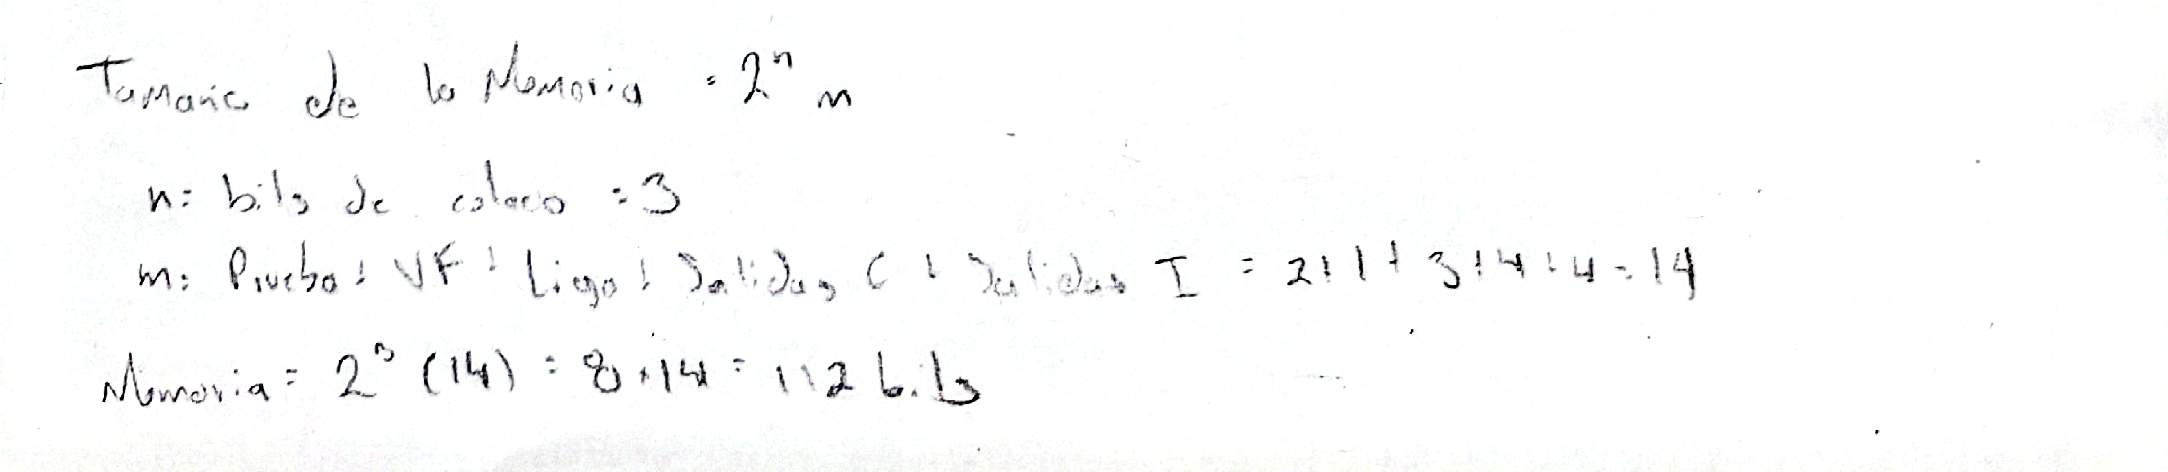
\includegraphics[width=0.9\textwidth,height=0.85\textheight,keepaspectratio]{evidencia-calculos.jpg}
  \caption{Cálculo manual inicial del tamaño de la memoria, con prueba de 2 bits.}
  \label{fig:evid-calc}
\end{figure}

\subsection{Contenido de la memoria}

La palabra se organiza como

\[
\text{dato} = \underbrace{\text{Prueba}}_{(14{:}12)} \ \Vert \
\underbrace{\text{VF}}_{(11)} \ \Vert \
\underbrace{\text{Liga}}_{(10{:}8)} \ \Vert \
\underbrace{\text{Salidas F}}_{(7{:}4)} \ \Vert \
\underbrace{\text{Salidas V}}_{(3{:}0)}
\]

Dentro de cada campo de salidas, los bits se ordenan como $S_1 S_2 \overline{U_1} \overline{U_2}$.
La tabla \ref{tab:memoria} presenta las ocho localidades, tal como se escribieron en el código
\texttt{memory.vhd}.

\begin{table}[htbp]
  \centering
  \caption{Contenido de la memoria con direccionamiento implícito. La dirección 111 no corresponde
  a un estado de la carta: su contenido de seguridad regresa a EST0.}
  \label{tab:memoria}
  \small
  \setlength{\tabcolsep}{5pt}
  \begin{tabular}{@{}c c c c c c@{}}
    \toprule
    \textbf{Dirección} & \textbf{Prueba} & \textbf{VF} & \textbf{Liga} & \textbf{Salidas F} & \textbf{Salidas V} \\
    \midrule
    000 (EST0) & 000 & 1 & 100 & 1001 & 1111 \\
    001 (EST1) & 001 & 0 & 001 & 0010 & 0110 \\
    010 (EST2) & 010 & 1 & 000 & 1001 & 1000 \\
    011 (EST3) & 100 & 0 & 000 & 0110 & 0110 \\
    100 (EST4) & 001 & 1 & 110 & 1111 & 1101 \\
    101 (EST5) & 000 & 1 & 000 & 0000 & 1000 \\
    110 (EST6) & 100 & 0 & 000 & 1100 & 1100 \\
    111 (sin uso) & 100 & 0 & 000 & 0011 & 0011 \\
    \bottomrule
  \end{tabular}
\end{table}

\subsection{Implementación en VHDL}

El sistema se describió en VHDL, repartido en nueve módulos más la entidad de nivel superior
\texttt{practica5}. La figura \ref{fig:bdf} presenta la misma interconexión vista como
esquemático de bloques en Quartus. El contador entrega la dirección \texttt{SAL[2..0]}, que direcciona la memoria. La
palabra leída se separa en prueba, VF, liga y salidas F y V. El selector de entradas \texttt{mux5}
toma la prueba y entrega la variable sensada; la compuerta XNOR la compara con VF y genera la señal
de carga, que gobierna el contador y el multiplexor de liga. El multiplexor de salidas, en
cambio, conmuta con el valor crudo de la variable sensada, de modo que las salidas falsas
se aplican cuando esa variable vale 0 y las verdaderas cuando vale 1.

\begin{figure}[H]
  \centering
  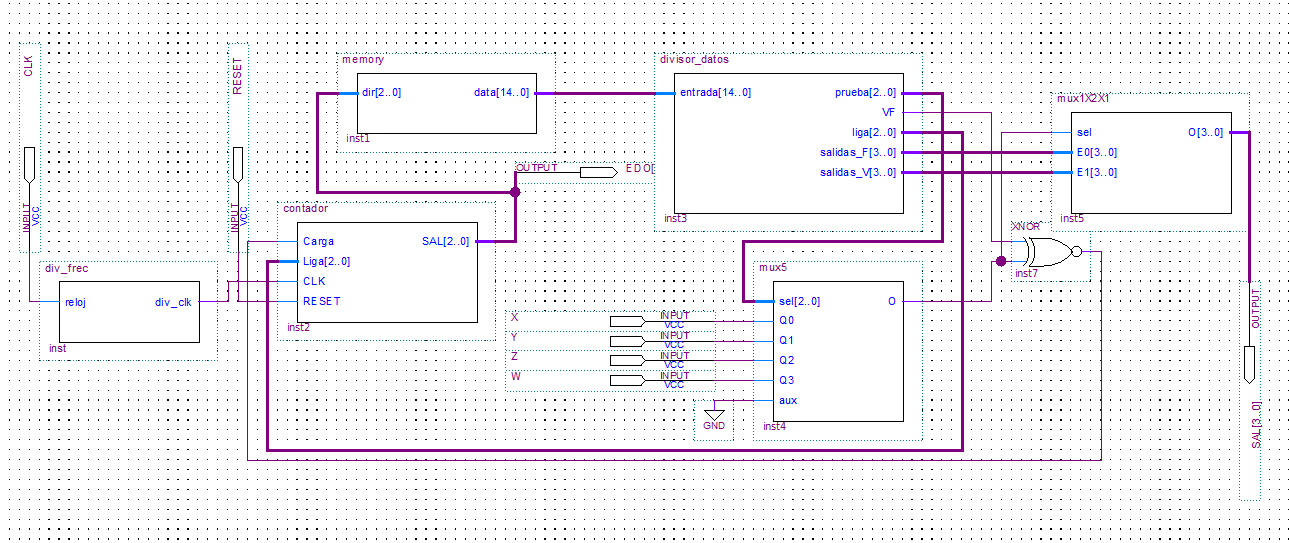
\includegraphics[width=\textwidth]{diagrama-bloques-p5.png}
  \caption{Esquemático en Quartus con la interconexión de los módulos.}
  \label{fig:bdf}
\end{figure}

El módulo \texttt{memory} implementa la ROM de 8 palabras de 15 bits.

\lstinputlisting[style=hdl]{codigo/memory.vhd}
\captionof{figure}{Código VHDL de la memoria con las ocho localidades del direccionamiento implícito.}
\label{fig:memory}

El módulo \texttt{divisor\_datos} separa la palabra leída en sus campos.

\lstinputlisting[style=hdl]{codigo/divisor_datos.vhd}
\captionof{figure}{Código VHDL del divisor que separa la palabra en prueba, VF, liga y salidas.}
\label{fig:divisor}

El módulo \texttt{mux5} es el selector de entradas. Su salida es la variable sensada, y la entrada
\texttt{aux} permite los saltos incondicionales.

\lstinputlisting[style=hdl]{codigo/mux5.vhd}
\captionof{figure}{Código VHDL del selector de entradas.}
\label{fig:mux5}

El módulo \texttt{mux1X2X1} selecciona entre las salidas F y V, y \texttt{mux1X2X1\_3} selecciona
entre el incremento y la liga del contador.

\lstinputlisting[style=hdl]{codigo/mux1X2X1.vhd}
\captionof{figure}{Código VHDL del selector de salidas (4 bits).}
\label{fig:mux1}

\lstinputlisting[style=hdl]{codigo/mux1X2X1_3.vhd}
\captionof{figure}{Código VHDL del selector de dirección (3 bits).}
\label{fig:mux13}

El módulo \texttt{incrementador} calcula el estado presente más uno.

\lstinputlisting[style=hdl]{codigo/incrementador.vhd}
\captionof{figure}{Código VHDL del incrementador.}
\label{fig:incr}

El módulo \texttt{register3} almacena el estado presente, con reset asíncrono activo en bajo.

\lstinputlisting[style=hdl]{codigo/register3.vhd}
\captionof{figure}{Código VHDL del registro de estado.}
\label{fig:register}

El módulo \texttt{contador} es el elemento secuencial del lazo. En cada flanco de reloj carga la liga
si la señal de carga está activa, o incrementa en uno en caso contrario.

\lstinputlisting[style=hdl]{codigo/contador.vhd}
\captionof{figure}{Código VHDL del contador con carga e incremento.}
\label{fig:contador}

Para observar el comportamiento en la tarjeta, un divisor de frecuencia reduce el reloj de 50~MHz a
una frecuencia de transición perceptible.

\lstinputlisting[style=hdl]{codigo/div_frec.vhd}
\captionof{figure}{Código VHDL del divisor de frecuencia.}
\label{fig:divfrec}

Finalmente, la entidad \texttt{practica5} instancia los módulos anteriores y los interconecta,
además de exponer el estado presente hacia los LEDs para poder observarlo.

\lstinputlisting[style=hdl]{codigo/practica5.vhd}
\captionof{figure}{Código VHDL de la entidad de nivel superior que interconecta los módulos.}
\label{fig:top}

\subsection{Asignación de pines}

Para la implementación en la tarjeta DE10-Lite (dispositivo MAX 10 10M50DAF484C7G) se realizó la
asignación de la tabla \ref{tab:pines}. Las entradas X, Y, Z y W se asignaron a los interruptores
SW0 a SW3, el \textit{reset} al botón \texttt{KEY0}, las salidas $S_1$, $S_2$, $\overline{U_1}$ y
$\overline{U_2}$ a \texttt{LEDR0} a \texttt{LEDR3}, y los tres bits del estado presente a
\texttt{LEDR9}, \texttt{LEDR8} y \texttt{LEDR7}.

\begin{table}[H]
  \centering
  \caption{Asignación de pines en la tarjeta DE10-Lite.}
  \label{tab:pines}
  \small
  \begin{tabular}{@{}l l l l@{}}
    \toprule
    \textbf{Señal} & \textbf{Pin} & \textbf{Recurso} & \textbf{Función} \\
    \midrule
    \texttt{CLK}     & \texttt{PIN\_P11} & \texttt{MAX10\_CLK1\_50} & Reloj de 50 MHz \\
    \texttt{RESET}   & \texttt{PIN\_B8}  & \texttt{KEY0}   & \textit{Reset} activo en bajo \\
    \texttt{X}       & \texttt{PIN\_C10} & \texttt{SW0}    & Entrada X \\
    \texttt{Y}       & \texttt{PIN\_C11} & \texttt{SW1}    & Entrada Y \\
    \texttt{Z}       & \texttt{PIN\_D12} & \texttt{SW2}    & Entrada Z \\
    \texttt{W}       & \texttt{PIN\_C12} & \texttt{SW3}    & Entrada W (no usada por la carta) \\
    \texttt{S1}      & \texttt{PIN\_A8}  & \texttt{LEDR0}  & Salida $S_1$ (activa en 1) \\
    \texttt{S2}      & \texttt{PIN\_A9}  & \texttt{LEDR1}  & Salida $S_2$ (activa en 1) \\
    \texttt{U1}      & \texttt{PIN\_A10} & \texttt{LEDR2}  & Salida $\overline{U_1}$ (activa en 0) \\
    \texttt{U2}      & \texttt{PIN\_B10} & \texttt{LEDR3}  & Salida $\overline{U_2}$ (activa en 0) \\
    \texttt{EDO[2]}  & \texttt{PIN\_B11} & \texttt{LEDR9}  & Bit 2 del estado presente \\
    \texttt{EDO[1]}  & \texttt{PIN\_A11} & \texttt{LEDR8}  & Bit 1 del estado presente \\
    \texttt{EDO[0]}  & \texttt{PIN\_D14} & \texttt{LEDR7}  & Bit 0 del estado presente \\
    \bottomrule
  \end{tabular}
\end{table}

\section{Análisis de resultados}

El proyecto se compiló en Quartus Prime 18.1.0 Lite Edition sin errores. La tabla
\ref{tab:sintesis} resume los recursos utilizados y el desempeño reportado por la herramienta.

\begin{table}[H]
  \centering
  \caption{Resumen de compilación del proyecto en Quartus Prime 18.1.}
  \label{tab:sintesis}
  \begin{tabular}{@{}l r@{}}
    \toprule
    \textbf{Parámetro} & \textbf{Valor} \\
    \midrule
    Elementos lógicos            & 62 / 49\,760 ($<1\%$) \\
    Registros dedicados          & 31 / 49\,760 ($<1\%$) \\
    Pines de E/S                 & 13 / 360 (4\%) \\
    Bits de memoria embebida     & 0 / 1\,677\,312 (0\%) \\
    $F_{max}$ (modelo 1200 mV, 85 $^\circ$C) & 168.75 MHz \\
    Errores de compilación       & 0 \\
    \bottomrule
  \end{tabular}
\end{table}

Dos cifras de la tabla \ref{tab:sintesis} merecen comentario. La primera es el conteo de 31
registros: 28 corresponden al contador del divisor de frecuencia y los 3 restantes al registro de
estado, lo que confirma que el único elemento secuencial del lazo de la máquina es ese registro.
La segunda es que la herramienta reporta cero bits de memoria embebida, ya que la ROM de 120 bits
no se mapeó a los bloques M9K del dispositivo sino que se sintetizó como lógica combinacional
dentro de los 62 elementos lógicos; esto es razonable dado su tamaño y no altera el comportamiento
del circuito. Los 168.75~MHz de frecuencia máxima superan ampliamente los 50~MHz del oscilador, de
modo que el diseño opera con holgura; la advertencia de incumplimiento temporal que emite el
analizador se debe únicamente a que el proyecto no incluye un archivo \texttt{.sdc}, y en ausencia
de restricciones Quartus asume un requisito por omisión de 1~GHz.

Antes de programar la tarjeta se verificó el comportamiento del diseño mediante simulación
funcional.

\subsection{Simulación funcional}

La simulación se compiló y ejecutó con GHDL, y la forma de onda se visualizó con GTKWave a partir del
archivo \texttt{sim.vcd}. El \textit{testbench} \texttt{tb\_practica5} instancia la cadena funcional
(memoria, divisor de datos, selector de entradas, selectores de salida y de dirección, y el contador)
y maneja las entradas X, Y, Z y W. Al ejecutarse, el banco de pruebas aplica 18 transiciones y compara
cada una con la carta ASM mediante sentencias \texttt{assert}. Al finalizar reporta: \textit{OK: las
18 transiciones y sus salidas coinciden con la carta ASM}.

\begin{figure}[H]
  \centering
  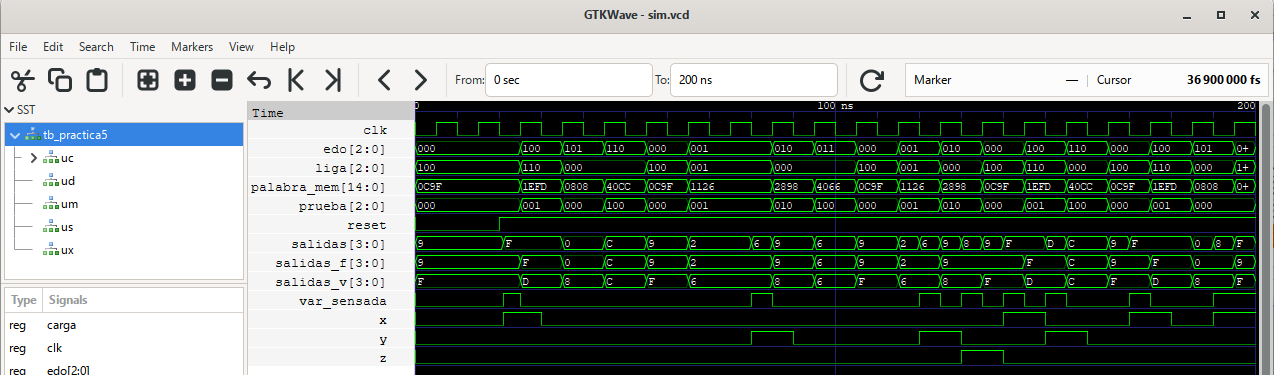
\includegraphics[width=\textwidth]{simulacion.png}
  \caption{Forma de onda de la simulación funcional. Se muestran el reloj, las entradas, el estado
  presente (\texttt{edo}), la palabra leída de memoria (\texttt{palabra\_mem}), la parte de prueba,
  la liga, la variable sensada y los tres juegos de salidas durante las 18 transiciones.}
  \label{fig:sim}
\end{figure}

\subsection{Verificación en la tarjeta}

Se programó la DE10-Lite con el diseño y se comprobó su funcionamiento en el laboratorio. La
máquina recorrió los estados de la carta ASM conforme a las condiciones de cada decisión, y las
salidas condicionales se activaron en los estados correspondientes. El funcionamiento se mostró a
la profesora durante la sesión.

\section{Conclusiones individuales}

\subsection{Omar Alfonso Zendejas Labias}

Con esta práctica entendí que el direccionamiento implícito cambia la forma en que la memoria decide
el siguiente estado. En lugar de guardar dos ligas, como en el método anterior, la palabra guarda una
sola liga y deja que el contador avance en uno cuando la condición no se cumple. Lo que más me sirvió
fue ver que la comparación entre la variable sensada y VF, hecha con una XNOR, es la que decide entre
incrementar y cargar, y que con ese mecanismo basta una sola liga por estado. También me quedó claro
que la carta debe construirse con los códigos consecutivos en las ramas de incremento, porque de lo
contrario la memoria no puede representar la transición.

Un punto que me ayudó a entender el método fue el error en mi cálculo manual. Al principio estimé
112 bits sin considerar los saltos incondicionales de EST3 y EST6. Al revisar la carta me di cuenta
de que esas transiciones necesitaban una entrada fija, y por eso el campo de prueba pasó a tener
3 bits y la memoria quedó en 120 bits. Esa corrección me mostró que el tamaño de la memoria depende
no solo de los estados y entradas, sino también de cómo se resuelven las transiciones sin condición.

\subsection{Emiliano García Olvera}

Considero que el objetivo de la práctica se cumplió. Con el direccionamiento implícito se implementó
una máquina de siete estados con tres entradas y cuatro salidas, usando una memoria de 8 localidades
de 15 bits, es decir, 120 bits en total (tabla \ref{tab:memoria}). La simulación con 18 transiciones
no presentó discrepancias respecto a la carta ASM, y el funcionamiento en la tarjeta coincidió con la
simulación, lo que confirma que el contenido de la memoria y la lógica de carga e incremento son
consistentes entre sí. Lo que más me aportó la práctica fue entender que las salidas condicionales se
obtienen desdoblando el campo de salidas en dos conjuntos y seleccionando uno de ellos con el valor de
la variable sensada, la misma que alimenta la XNOR que decide el siguiente estado.

\renewcommand{\refname}{Bibliografía}
\begin{thebibliography}{9}
\bibitem{savage} J. Savage Carmona, G. Vázquez y N. E. Chávez Rodríguez,
  \emph{Diseño de microprocesadores}. Ciudad de México, México: Facultad de Ingeniería,
  Universidad Nacional Autónoma de México, 2017. [En línea]. Disponible:
  \url{http://profesores.fi-b.unam.mx/luist/archivos/MicroprocesadoresSavage.pdf}
\bibitem{mano} M. M. Mano y M. D. Ciletti, \emph{Diseño digital}, 5a ed.
  Naucalpan de Juárez, México: Pearson Educación, 2013.
\end{thebibliography}

\end{document}